\chapter{Uitwendige stroming}
\label{sec:Uitwendige stroming}

%%%%%%%%%%%%%%%%%%%%%%%%%%%%%%%%%%%%%%%%%%%%%%%%%%%%%%%%%%%%%%%%%%%%%%%%%%%%%%%%%%%%%
	\section{Inleiding}
	\label{sec:Uitwendige stroming Inleiding}
In dit hoofdstuk zullen een aantal hulpiddelen voor het beschijven van stroming uitwendig aan een voorwerp beschreven worden. Als eerste wordt een analytische methode voor niet viskeuze tweedimensionale stroming besproken. Nadien wordt het gedrag van een viskeuze uitwendige stroming beschreven. In het laatste deel wordt de stroming rond een vleugelprofiel, een in de ingenieurstoepassing vaak voorkomende vorm, beschreven.

%%%%%%%%%%%%%%%%%%%%%%%%%%%%%%%%%%%%%%%%%%%%%%%%%%%%%%%%%%%%%%%%%%%%%%%%%%%%%%%%%%%%%
	\section{Potentiaalstroming}
	\label{sec:Potentiaalstroming}

Uit de vectorveld analyse weten we dat wanneer een vectorveld rotatievrij is er een scalaire potentiaalfunctie bestaat waaruit de componenten van het vectorveld kunnen worden afgeleid.

Wanneer er geen viskeuze krachten op een fluïdum inwerken zal de rotatie van het snelheidsveld $0$ zijn. Het met andere woorden: het snelheidsveld is rotatievrij. Er zal dus een potentiaalfunctie bestaan waaruit de componenten van het snelheidsveld kunnen worden afgeleid.

Dit vereenvoudigt de oplossing van het snelheidsveld voor gegeven randvoorwaarden aanzienlijk. Voor een tweedimensionale niet-samendrukbare stroming moet normaal gezien een stelsel van 3 gekoppelde partiële differentiaalvergelijkingen opgelost worden (één voor elke richting en de continuïteitsvergelijking). Onder de voorwaarden van potentiaalstroming vereenvoudigt dit tot één partiële differentiaalvergelijking.
		\subsection{Stroomfunctie}
Beschouw een willekeurige tweedimensionale stroming met stroomlijnen zoals in Figuur \ref{fig:Stroomfunctie}.
\begin{figure}[htb]
	\centering
	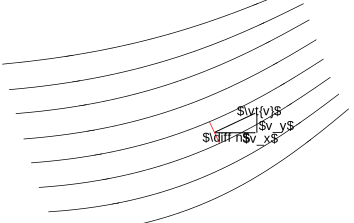
\includegraphics{fig/uitwendige_stroming/Stroomfunctie}
	\caption{Stroomlijnen van een tweedimensionale stroming}
	\label{fig:Stroomfunctie}
\end{figure}
Berekenen we nu het debiet $\diff \dot{V}$ tussen twee stroomlijnen op een afstand $\diff n$.
\begin{equation}
	\diff \dot{V} = v \diff n
\end{equation}
De snelheid kan beschreven worden door zijn 2 componenten, $v_x$ en $v_y$. We kunnen de vector $\diff n$ beschrijven met zijn componenten $dx$ en $dy$ (Figuur \ref{fig:Stroomlijn coordinaten}). De componenten van $\vt{v}$ loodrecht op het oppervlak $\diff n$ kunnen nu berekend worden als:
\begin{eqnarray}
	v_{x,\perp} &=&  v_x \frac{\diff y}{\diff n} \\
	v_{y,\perp} &=& -v_y \frac{\diff x}{\diff n}
\end{eqnarray}
Hierin wordt bij $\diff x$ een min teken toegevoegd aangezien $\diff x$ zoals hier getekend een negatieve waarde zal hebben. Het debiet wordt nu:
\begin{equation}
	\diff \dot{V} = v_x \frac{\diff y}{\diff n} \diff n - v_y \frac{\diff x}{\diff n} \diff n = v_x \diff y - v_y \diff x
	\label{eqn:debiet tussen stroomlijnen}
\end{equation}
Beschouw nu de onbekende stroomfunctie $\psi$ die een scalaire functie is in $x$ en $y$. De verandering van deze stroomfunctie kan met behulp van de kettingregel geschreven worden in functie van zijn partiële afgeleiden naar de twee co\"ordinaten:
\begin{equation}
	\diff \psi = \frac{\partial \psi}{\partial x} \diff x + \frac{\partial \psi}{\partial y} \diff y
	\label{eqn:verandering van de stroomfunctie}
\end{equation}
Indien we nu (\ref{eqn:debiet tussen stroomlijnen}) en (\ref{eqn:verandering van de stroomfunctie}) vergelijken zien we dat we de stroomfunctie kunnen definiëren als het debiet tussen een stroomlijn en een vaste referentie stroomlijn. De snelheidscomponenten kunnen dan uit de stroomfunctie afgeleid worden als:
\begin{eqnarray}
	v_x &=&  \frac{\partial \psi}{\partial y} \\
	v_y &=& -\frac{\partial \psi}{\partial x}
\end{eqnarray}
\begin{figure}[htb]
	\centering
	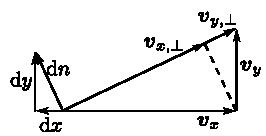
\includegraphics{fig/uitwendige_stroming/Stroomlijnen}
	\caption{Vectoren van de stroomlijn co\"ordinaten}
	\label{fig:Stroomlijn coordinaten}
\end{figure}
Een belangrijke eigenschap van de stroomfunctie is dat contouren van constante stroomfunctie de stroomlijnen beschrijven. Dit kan rechtstreeks afgeleid worden uit de interpretatie van de stroomfunctie als debiet.

Uit de vector analyse volgt dat voor een rotatievrije stroming de stroomfunctie moet voldoen aan de Laplacevergelijking.
\begin{equation}
	\frac{\partial^2 \psi}{\partial x^2} + \frac{\partial^2 \psi}{\partial y^2} = 0
	\label{eqn:laplacevergelijking}
\end{equation}
Analytische oplossingen voor deze vergelijking bestaan voor een groot aantal verschillende randvoorwaarden. Een bijkomend voordeel van deze formulering is dat de Laplacevergelijking een lineaire partiële differentiaalvergelijking is. Hierop is het superpositieprincipe van toepassing. Een lineaire combinatie van oplossingen zal dus ook voldoen aan de vergelijking. Met behulp hiervan kunnen een aantal problemen analytisch behandeld worden.

\begin{voorbeeld}
	\label{Potentiaalstroming_cilinder}
	Bepaal en teken de stroomlijnen voor een stroming met snelheid $v_{\infty}$ rond een cilinder met straal $R$.
	\begin{center}
		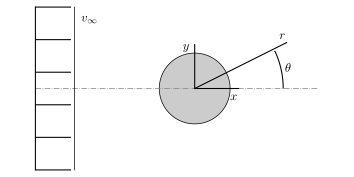
\includegraphics{Potentiaalstroming_cilinder}
	\end{center}
	
	De stroomfunctie voor de stroming rond een cilinder kan worden gevonden door de superpositie van een uniforme stroming en een doublet. Aangezien we rond een cilinder werken is het aangewezen om in poolcoordinaten te werken. De stroomfunctie van een uniforme stroming wordt dan:
	\begin{equation*}
		\psi = v_{\infty} r \sin{\theta}
	\end{equation*}
	Een doubles wordt gevormd wanneer een bron van fluïdum en een put infinitesimaal dicht bij elkaar geplaatst worden. De stroomfunctie kan geschreven worden als:
	 \begin{equation*}
		\psi = -\frac{K \sin \theta}{r}
	\end{equation*}
	De stroomlijnen zien er als volgt uit:
	\begin{center}
		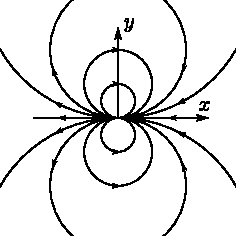
\includegraphics{Potentiaalstroming_doublet}
	\end{center}
	De gezochte stroomfunctie wordt dus:
	\begin{equation*}
		\psi = v_{\infty} r \sin{\theta} - \frac{K \sin \theta}{r}
	\end{equation*}

	De sterkte van het doublet $K$ moet zo gekozen worden zodat de cilinderomtrek een stroomlijn is. Dit betekent dat op $r=R$, $v_r$ nul moet zijn met de partieel afgeleiden in cilindercoördinaten wordt de radiale snelheid:
	\begin{align*}
		v_{r} &= \dfrac{1}{r}\dfrac{\partial \psi}{\partial \theta} \\
		      &= v_{\infty} \cos{\theta} - \frac{K \cos \theta}{r^2}
	\end{align*}
	Dus op de cilindermantel:
	\begin{align*}
		0 &= v_{\infty} \cos{\theta} - \frac{K \cos \theta}{R^2}
		  &= v_{\infty} \cos{\theta} R^2 - K \cos \theta
		K &= v_{\infty} R^2
	\end{align*}
	De stroomfunctie wordt:
	\begin{equation*}
		\psi = v_{\infty} r \sin{\theta} - \frac{v_{\infty} R^2 \sin \theta}{r}
	\end{equation*}
	De stroomlijnen kunnen nu getekend worden:
	\begin{center}
		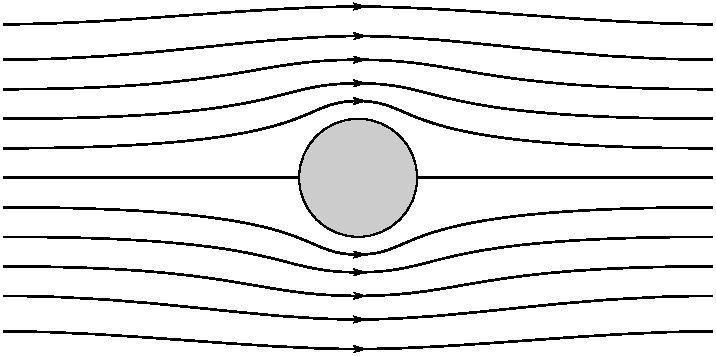
\includegraphics{Potentiaalstroming_cilinder_stroomlijnen}
	\end{center}
	
\end{voorbeeld}

%%%%%%%%%%%%%%%%%%%%%%%%%%%%%%%%%%%%%%%%%%%%%%%%%%%%%%%%%%%%%%%%%%%%%%%%%%%%%%%%%%%%%
	\section{Grenslagen}
	\label{sec:Grenslagen}
Beschouw vlakke plaat waar langs één zijde een viskeus fluïdum over stroomt (Figuur \ref{fig:Laminaire grenslaag}). Vlak voor de plaat is de stroming uniform, de snelheid varieert niet met de hoogte. Bij het begin van de plaat zullen de deeltjes het dichtst bij de plaat door de wrijvingskrachten afgeremd worden tot stilstand. De deeltjes verder van de plaat worden op deze plaats echter nog niet beïnvloed door de plaat. Wanneer het fluïdum verder over de plaat stoomt zullen de deeltjes die iets verder van de plaat stromen ook afgeremd worden door de deeltjes het dischtst bij de plaat. De deeltjes ver van de plaat ondervinden echter nog steeds geen invloed van de plaat.
\begin{figure}[htb]
	\centering
	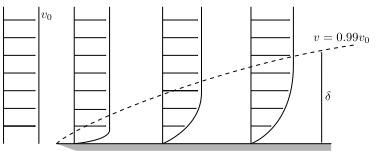
\includegraphics{fig/uitwendige_stroming/Laminaire_grenslaag}
	\caption{Vorming van een grenslaag bij stroming over een vlakke plaat}
	\label{fig:Laminaire grenslaag}
\end{figure}

Hoe verder we van het begin van de plaat kijken hoe groter de zone waarin de fuiïdum deeltjes het effect van de plaat ondervinden zal worden. De zone waarin de snelheid van het fuiïdum kleiner is dan 99\% van de ongestoorde snelheid wordt de \emph{grenslaag} genoemd.

Bij elke viskeuze stroming die in aanraking komt met een wand op een andere snelheid wordt een grenslaag gevormd. Deze vormt een handig hulpmiddel voor de analyse van viskeuze stromingen rond voorwerpen aangezien slechts een gedeelte van het stroomveld in rekening gebracht moet worden (het gedeelte binnen de grenslaag). De bepaling van de dikte van een grenslaag is echter niet zo eenvoudig en zal niet behandeld worden in deze cursus.

Wanneer de dikte van de grenslaag echter gekend is kan gemakkelijk een snelheidsprofiel verondersteld worden. Hieruit kunnen dan de schuifspanningen aan de wand berekend worden en uit deze volgt de viskeuze weerstandskracht die de vloeistof op de wand uitoefent.

In het voorgaande voorbeeld liepen alle snelheidsvectoren in dezelfde richting. Indien we de stroomlijnen in deze stroming zouden tekenen is te zien dat deze allemaal parallel lopen. De stroming wordt als het ware door de ongestoorde snelheid gedwongen in verschillende lagen te stromen. Zo'n stroming noemen we \emph{laminair}. Wanneer we ons nog verder over de wand verplaatsen zal de grenslaag steeds dikker worden. Op een gegeven moment wordt de grenslaag zo dik dat de stroming binnen de grenslaag onstabiel wordt. Er zullen variaties van de grootte en richting van de snelheid optreden naargelang de plaats en het tijdstip waarop we kijken (Figuur \ref{fig:Turbulente grenslaag}). We noemen dit een turbulente grenslaag.
\begin{figure}[htb]
	\centering
	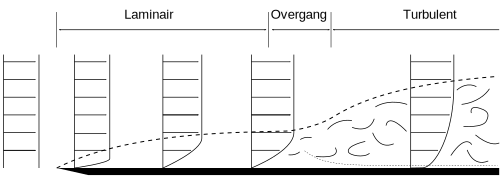
\includegraphics{fig/uitwendige_stroming/Turbulente_grenslaag}
	\caption{Vorming van een turbulente grenslaag bij stroming over een vlakke plaat}
	\label{fig:Turbulente grenslaag}
\end{figure}

In een turbulente grenslaag zal het fluïdum niet meer netjes in lagen stromen. Zeer dicht bij de wand zal er wel een kleine zone van laminaire stroming zijn. Hier zorgt de wand voor de stabilisatie van de stroming. We noemen deze laag de laminaire sublaag.

In een turbulente grenslaag wordt de weerstandskracht niet enkel meer bepaald door de viscositeit. Buiten de laminaire sublaag beweegt de vloeistof onregelmatig door elkaar. Er zal dus convectieve impulsoverdracht plaatsvinden over de lagen heen. De schuifspanning wordt hier veroorzaakt door de onregelmatigheid van de snelheden en wordt de turbulente schuifspanning of Reynoldsspanning genoemd. Het correct bepalen van deze spanningen is tot op heden niet mogelijk en vormt één van de blijvende uitdagingen in de fluïdummechanica. Er bestaan wel meerdere ad hoc benaderingen voor de Reynoldsspanningen die in bepaalde gevallen voldoende betrouwbare resultaten geven.

Binnen de laminaire sublaag zal de laminaire schuifspanning terug domineren. Aangezien er in het turbulente gedeelte meer impuls overdracht is zal een turbulent snelheidsprofiel steeds een grotere gradiënt hebben in de buurt van de wand en vlakker zijn verder van de wand. De uitgeoefende viskeuze weerstandskracht is dan ook steeds groter bij een turbulente stroming dan bij een laminaire stroming.


		\subsection{Het snelheidsprofiel van een laminaire stroming over een vlakke plaat}
Beschouw een niet-samendrukbare, laminaire stroming van een newtoniaanse vloeistof over een vlakke plaat. Deze stroming voldoet aan de Navier-Stokes vergelijking (\ref{eqn:navier-stokes vergelijkingen carthesiaans}). Indien we de stroming als stationair beschouwen en het effect van de zwaartekracht verwaarlozen wordt dit:
\begin{eqnarray}
	v_x \frac{\partial v_x}{\partial x} + v_y \frac{\partial v_x}{\partial y} &=& -\frac{1}{\rho}\frac{\partial p}{\partial x} + \nu \left( \frac{\partial^2 v_x}{\partial x^2} + \frac{\partial^2 v_x}{\partial y^2} \right) \\
	v_x \frac{\partial v_y}{\partial x} + v_y \frac{\partial v_y}{\partial y} &=& -\frac{1}{\rho}\frac{\partial p}{\partial y} + \nu \left( \frac{\partial^2 v_y}{\partial x^2} + \frac{\partial^2 v_y}{\partial y^2} \right)
\end{eqnarray}
De continuïteitsvergelijking (\ref{eqn:continuiteitsvergelijking}) in differentiaalvorm wordt:
\begin{equation}
	\frac{\partial v_x}{\partial x} + \frac{\partial v_y}{\partial y} = 0
\end{equation}
Wanneer we de randvoorwaarden toevoegen dat ver van de wand de snelheid de vrije stroomsnelheid $v_0$ is en op aan de wand de snelheid 0 is, hebben we voldoende voorwaarden om het probleem op te lossen. Er is echter nog geen analytische oplossing gevonden voor dit probleem. Om het probleem op te lossen moeten we enkele vereenvoudigingen invoeren. 

Aangezien de grenslaag zich dicht tegen de plaat bevind is het aannemelijk dat de snelheid in de richting loodrecht op de plaat ($v_y$), veel kleiner is dan de snelheid in de richting van de plaat ($v_x$). Ook zal de verandering van variabelen in de loodrechte richting ($\frac{\partial}{\partial y}$) veel kleiner zijn de de verandering in de stroomrichting ($\frac{\partial}{\partial x}$). Uit experimenten weten we ook dat de druk in de volledige stroming ongeveer constant is. 

Met deze vereenvoudigingen zal de impuls vergelijking in de $y$-richting niet meer belangrijk zijn. In de impulsvergelijking in de $x$-richting kunnen we de drukterm schrappen. Aangezien in de viskeuze kracht term de tweede afgeleide naar $y$ staat en deze veel kleiner is dan de tweede afgeleide naar $x$ kunnen we ook deze schrappen. De impulsvergelijking in de $x$-richting wordt dan:
\begin{equation}
	v_x \frac{\partial v_x}{\partial x} + v_y \frac{\partial v_x}{\partial y} = \nu \left( \frac{\partial^2 v_x}{\partial x^2} \right) \\
\end{equation}
De randvoorwaarden worden:
\begin{eqnarray}
	v_x|_{y=0} = v_y|_{y=0} &=& 0 \\
	v_x|_{y\rightarrow\infty} &=& v_0
\end{eqnarray}

Deze partiële differentiaalvergelijking kan door middel van een coördinaten transformatie omgevormd worden tot een gewone differentiaal vergelijking die eenvoudig numeriek kan opgelost worden. De uitwerking hiervan werd het eerst gedocumenteerd door Paul Richard Heinrich Blasius in 1908 maar valt buiten het bereik van deze cursus geïnteresseerde lezers worden verwezen naar \cite{Schlichting1979} waar dit probleem en vele andere grenslaag problemen zeer goed uitgewerkt worden.

De numeriek oplossing gebruikt een getransformeerde coördinaat $\eta = y (\frac{v_0}{\nu x})^{1/2}$. De relatieve snelheid in de grenslaag in functie van deze coördinaat wordt gegeven in Figuur  \ref{fig:Grenslaagsnelheid}. Merk op dat deze figuur kan gebruikt worden om de snelheid in de grenslaag op alle hoogtes en alle afstanden van de rand van de plaat te berekenen aangezien de coördinaat $\eta$ zowel de $y$ als $x$ coördinaat bevat.
\begin{figure}[htb]
	\centering
	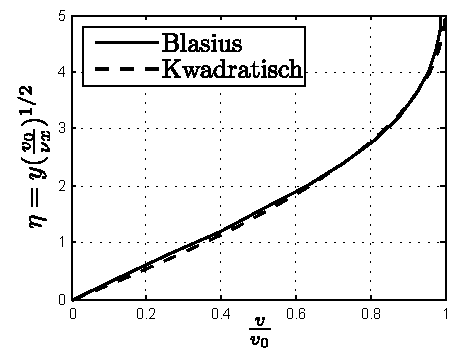
\includegraphics{fig/uitwendige_stroming/Grenslaagsnelheid}
	\caption{Blasius oplossing van de snelheid in de grenslaag bij laminaire stroming over een vlakke plaat}
	\label{fig:Grenslaagsnelheid}
\end{figure}

Uit de Figuur \ref{fig:Grenslaagsnelheid} valt af te leiden dat de grenslaagdikte (de positie waar de relatieve snelheid 0.99 is) overeenkomt met $\eta = 5$. Hieruit kunnen we het verloop van grenslaagdikte met de afstand tot het aanstroompunt bepalen:
\begin{equation}
	\delta = 5 \sqrt{\frac{\nu x}{v_0}}
\end{equation}

Aangezien het snelheidsprofiel volgens Blasius geen analytische uitdrukking heeft is het niet eenvoudig om berekeningen mee uit te voeren. We kunnen het snelheidsprofiel echter zeer goed benaderen met een kwadratisch snelheidsprofiel zoals getoond in Figuur \ref{fig:Grenslaagsnelheid}. Dit benaderende snelheidsprofiel kunnen we uitdrukken als:
\begin{equation}
	\delta = \frac{2}{5}\eta - \frac{1}{25}\eta^2
\end{equation}

		\subsection{Impulsbalans voor de laminaire stroming over een vlakke plaat}
		\label{sec:Impulsbalans voor de laminaire stroming over een vlakke plaat}
Voor een laminaire stroming over een vlakke plaat kunnen we de weerstandskracht uitwerken door een controlevolume te beschouwen rond de grenslaag. Kies als randen voor het controle volume de vlakke plaat zelf, een verticale aan het begin van de plaat, een verticale op de beschouwde positie $x$ en een stroomlijn die op positie $x$ door de rand van de grenslaag stroomt. Ter hoogte van het begin van de plaat bevindt deze stroomlijn zich op een hoogte $h$ (Figuur \ref{fig:Laminaire_genslaag_controlevolume}).
\begin{figure}[htb]
	\centering
	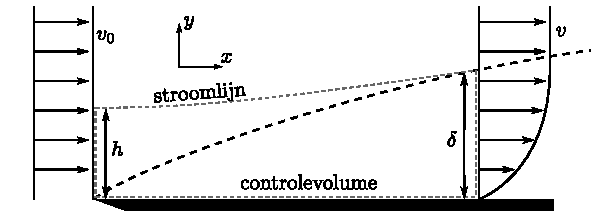
\includegraphics{fig/uitwendige_stroming/Laminaire_grenslaag_controlevolume}
	\caption{Controle volume in de laminaire stroming over een vlakke plaat voor de berekening van de weerstandskracht}
	\label{fig:Laminaire_genslaag_controlevolume}
\end{figure}

We kunnen nu de impulsbalans voor dit controlevolume in de $x$-richting uitschrijven. Aangezien het een stationair controlevolume met één ingang en één uitgang is wordt dit:
\begin{equation}
	F_x = \int_0^{\delta} \rho v(y)^2 b \diff y  - \int_0^{h} \rho v_0^2 b \diff y
	\label{eqn:laminaire grenslaag impuls}
\end{equation}
Hierin stelt b de breedte van de plaat voor. De krachten die inwerken op de het controlevolume zijn de schuifspanning aan de wand $\tau_w$, de druk aan de in en uitlaat, en de druk ter hoogte van de stroomlijn. Uit experimenten weten we dat de druk in de volledige stroming constant is. De druk zal dus geen resulterende kracht uitoefenen op het controlevolume. De totale kracht uitgeoefend op het controlevolume is dan het negatieve van de weerstandskracht uitgeoefend op de plaat:
\begin{equation}
	F_x = -F_d = -\int_0^x \tau_w b \diff x
\end{equation}

Om de hoogte $h$ van de stroomlijn aan het begin van de plaat te berekenen kunnen we de massabalans opstellen. Na vereenvoudiging wordt dit:
\begin{equation}
	\rho v_0 b h = \int_0^{\delta} \rho v(y) b \diff y
\end{equation}
Indien we beide leden vermenigvuldigen met $v_0$ bekomen we in het linker lid een uitdrukking die gelijk is aan de tweede term in het rechterlid van (\ref{eqn:laminaire grenslaag impuls}). Na invullen van bovenstaande resultaten wordt dit:
\begin{equation}
	-F_d = \int_0^{\delta} \rho v(y)^2 b \diff y  - \int_0^{\delta} \rho v_0 v(y) b \diff y
\end{equation}
In het rechterlid van deze vergelijking kunnen we de integralen combineren tot:
\begin{equation}
	F_d = \rho b \int_0^{\delta} v(y)(v_0-v(y))\diff y
\end{equation}
Deze vergelijking illustreert dat de weerstandskracht door viskeuze wrijving gebalanceerd wordt door een impuls daling in de grenslaag. Hoe verder we ons op de plaat bewegen hoe meer weerstand er zal uitgeoefend worden. De totale impuls in de grenslaag moet dus dalen en als gevolg van behoud van massa zal de grenslaag dikte groter worden.

		\subsection{Turbulentie}
Wanneer het Reynoldsgetal in een stroming groot genoeg is zal de stroming turbulent worden. Het snelheidsveld dat de stroming beschrijft bevat dan schijnbaar willekeurige variaties in grootte en richting van de snelheid. Het fenomeen werd als eerste beschreven en gekwantificeerd door Osbourne Reynolds voor een stroming in een buis. Een turbulente stroming wordt gekarakteriseerd door:
\begin{itemize}
	\item Wanordelijke, schijnbaar willekeurige stroming
	\item Zeer gevoelig aan begincondities
	\item Grote menging en dissipatie
	\item Grote variatie in lengte en tijdschalen
	\item 3 dimensionaal
\end{itemize}

Wanneer in een stroming energie toegevoegd wordt op een grote lengte schaal zal deze energie door wervelingen overgedragen worden naar steeds kleinere lengteschalen, tot een schaal waar de viscositeit overheerst en de energie gedissipeerd wordt tot warmte door viskeuze wrijving. Dit principe werd in 1922 poëtisch beschreven door Lewis Fry Richardson:
\begin{quotation}
Big whorls have little whorls,\\
which feed on their velocity;\\
And little whorls have lesser whorls\\
and so on to viscosity.\\
\end{quotation}

Dit principe kan geillustreerd worden aan de hand van een grote tank met een roer installatie (Figuur \ref{fig:Energie_cascade}). De roerder voegt energie toe en creërt een grote wervel op de schaal van de tank zelf. Deze wervel zal zijn energie overdragen aan kleinere wervels met hogere snelheid, die op hun beurt de energie overdragen aan nog kleinere wervels. Dit proces gaat door to de lengte schaal zo klein is en de snelheid zo groot dat de viscositeit terug domineert en de mechanische energie omgezet wordt in warmte. Dit principe noemt men ook de energie cascade.
\begin{figure}[htb]
	\centering
	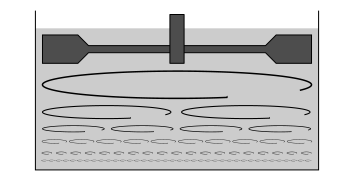
\includegraphics{fig/uitwendige_stroming/Energie_cascade}
	\caption{Illustratie van de energie cascade bij een turbulente menging in een tank waarbij energie toegevoegd wordt door een roerder.}
	\label{fig:Energie_cascade}
\end{figure}

De oorzaak van de energiecascade kunnen we illustreren met een eenvoudig voorbeeld. Beschouw een stroming met een sinusvormige verstoring in de $x$-richting ($v_x = \sin(\omega x)$). De convectieve term van de deeltjesversnelling in de $x$-richting wordt nu:
\begin{equation}
	v \frac{\partial v}{\partial x} = \omega \sin(\omega x) \cos(\omega x) = \frac{1}{2} \omega \sin( 2 \omega x) 
\end{equation}
Een aanwezige verstoring wordt dus met een half zo kleine golflengte overgedragen naar de versnelling. Er wordt dus een nieuwe verstoring gecreerd met een kleinere golflengte en hogere frequentie. Hierdoor zal een globale verstoring evolueren tot een variatie in snelheid op zeer kleine schaal.

Een turbulente stroming wordt nog steeds beschreven door de Navier-Stokes vergelijking (\ref{eqn:navier-stokes vergelijkingen}). Door de niet lineaire convectieve termen in de deeltjesversnelling ($v_i \frac{\partial v_j}{\partial x_i}$) is het bekomen van een oplossing voor de vergelijkingen tot nog toe niet mogelijk. Wel bestaan er technieken die het numeriek benaderen van turbulente stroming mogelijk maken.

Het Reynolds getal (verhouding tussen traagheidskrachten en viskeuze krachten) is een goede maatstaf voor het inschatten van turbulentie. De Reynoldsgetallen waarbij turbulentie optreedt zijn echter sterk afhankelijk van de specifieke situatie. Bij de grenslaagstroming over een vlakke plaat zoals hierboven beschreven zal turbulentie optreden vanaf een Reynoldsgetal van 350000 - 1000000 \cite{Schlichting1979}. Het Reynoldsgetal word in dit geval gedefinieerd als:
\begin{equation}
	Re_x = \frac{v x}{\nu}
\end{equation}
Hierin is $x$ de afstand van het beschouwde punt tot de rand van de plaat. Een voorbeeld van de ogenblikkelijke snelheidsvectoren van een turbulente stroming over een vlakke plaat is gegeven in Figuur \ref{fig:Turbulente grenslaag voorbeeld}.
\begin{figure}[htb]
	\centering
	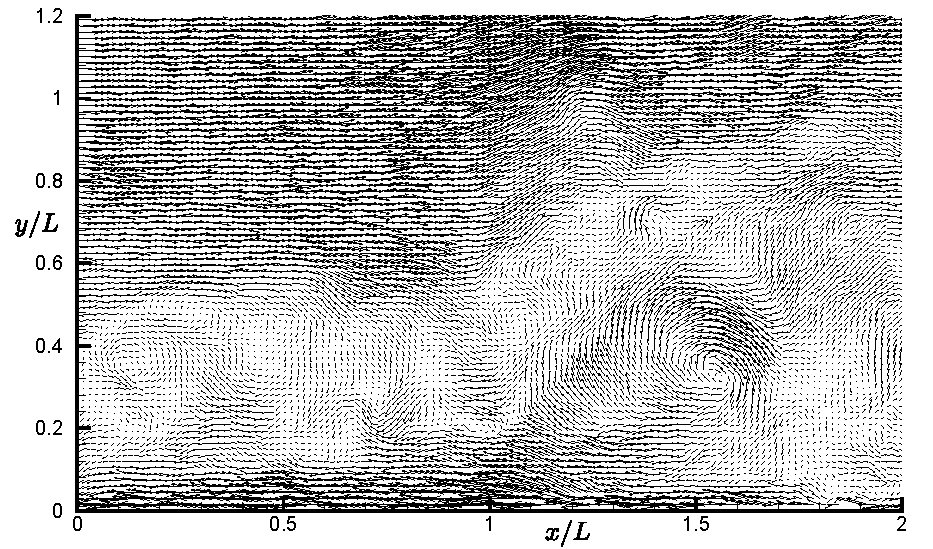
\includegraphics[width=15cm]{fig/uitwendige_stroming/Turbulente_grenslaag_voorbeeld}
	\caption{Ogenblikkelijke snelheidsvectoren opgemeten bij een turbulente grenslaag over een vlakke plaat \cite{Tomkins1997}.}
	\label{fig:Turbulente grenslaag voorbeeld}
\end{figure}

Meer informatie over turbulentie is te vinden in \cite{McDonough2007}.

%%%%%%%%%%%%%%%%%%%%%%%%%%%%%%%%%%%%%%%%%%%%%%%%%%%%%%%%%%%%%%%%%%%%%%%%%%%%%%%%%%%%%
	\section{Loshechting}
	\label{sec:Loshechting}
	
Beschouw de stroming rond een cilinder. Wanneer we de stroomlijnen tekenen voor verschillende Reynolds getallen kunnen we enkel duidelijke regimes onderscheiden (Figuur \ref{fig:Sroomlijnen bij stroming rond een cilinder}).

Bij zeer lage snelheden zullen de viskeuze krachten overheersen (Figuur \ref{fig:cilinder Re 1} en Figuur \ref{fig:cilinder Re 10}). De stroming is zeer viskeus en de snelheid zal in het gehele stroomveld het effect van de cilinder ondervinden. De grenslaag is in dit geval zeer groot.
We kunnen een wrijvingscoëfficiënt berekenen als:
\begin{equation}
	C_d = \frac{F_d}{1/2 \rho v^2 A_{\perp}}
	\label{eqn:wrijvingscoefficient}
\end{equation}
Deze zal bij lage Reynoldsgetallen zeer groot zijn en sterk afhankelijk zijn van het Reynoldsgetal (Figuur \ref{fig:cilinderstroming_cd}). De wrijving wordt echter slechts gedeeltelijk door viskeuze wijving (ten gevolge van de grenslaag) veroorzaakt. Het overige gedeelte wordt veroorzaakt door het drukverschil tussen de voor en achterzijde.
\begin{figure}[htb]
	\centering
	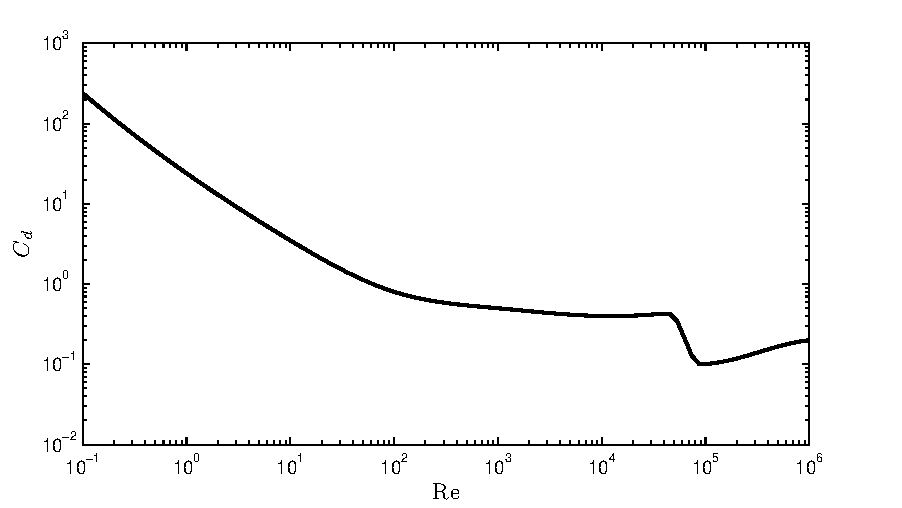
\includegraphics{cilinderstroming_Cd.pdf}
	\caption{Wrijvingsfactor bij stroming van rond een cilinder }
	\label{fig:cilinderstroming_cd}
\end{figure}
\begin{figure}[htb]
	\centering
	\includegraphics{fig/uitwendige_stroming/loshechting}
	\caption{Afscheiding van een viskeuze stroming onder invloed van een positieve drukgradiënt}
	\label{fig:afscheiding}
\end{figure}
\begin{figure}[htb]
	\centering
	\subfigure[Re = 1]{
		\label{fig:cilinder Re 1}
		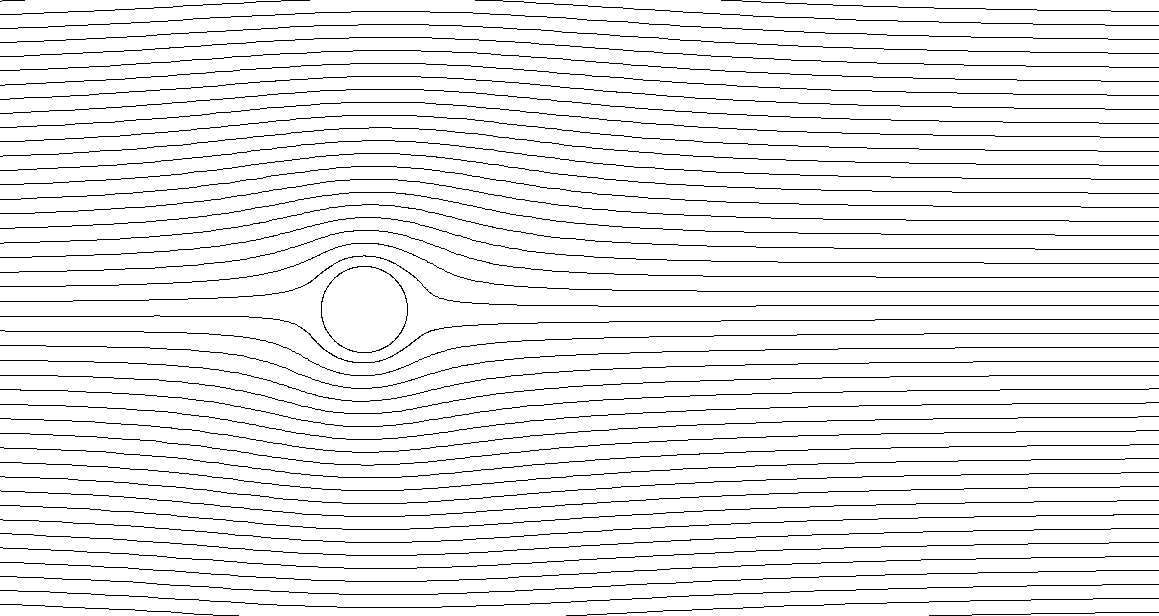
\includegraphics[height=0.2\textwidth]{Stroomfunctie_Re1_bw.png}
	} \quad
	\subfigure[Re = 10]{
		\label{fig:cilinder Re 10}
		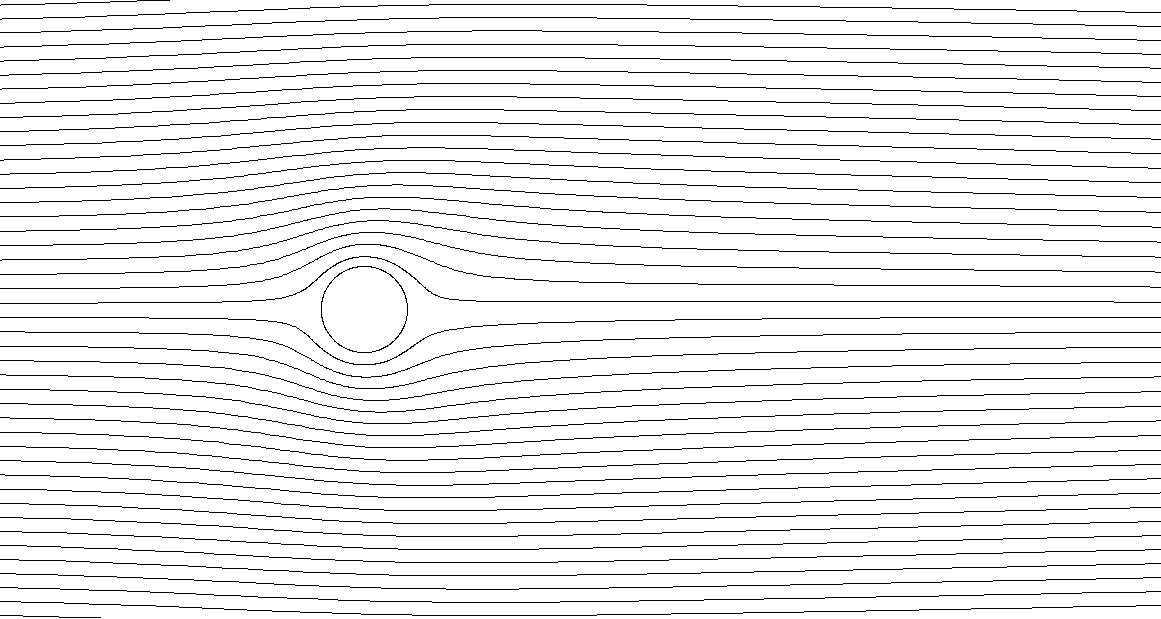
\includegraphics[height=0.2\textwidth]{Stroomfunctie_Re10_bw.png}
	}
	\\
	\subfigure[Re = 100]{
		\label{fig:cilinder Re 100}
		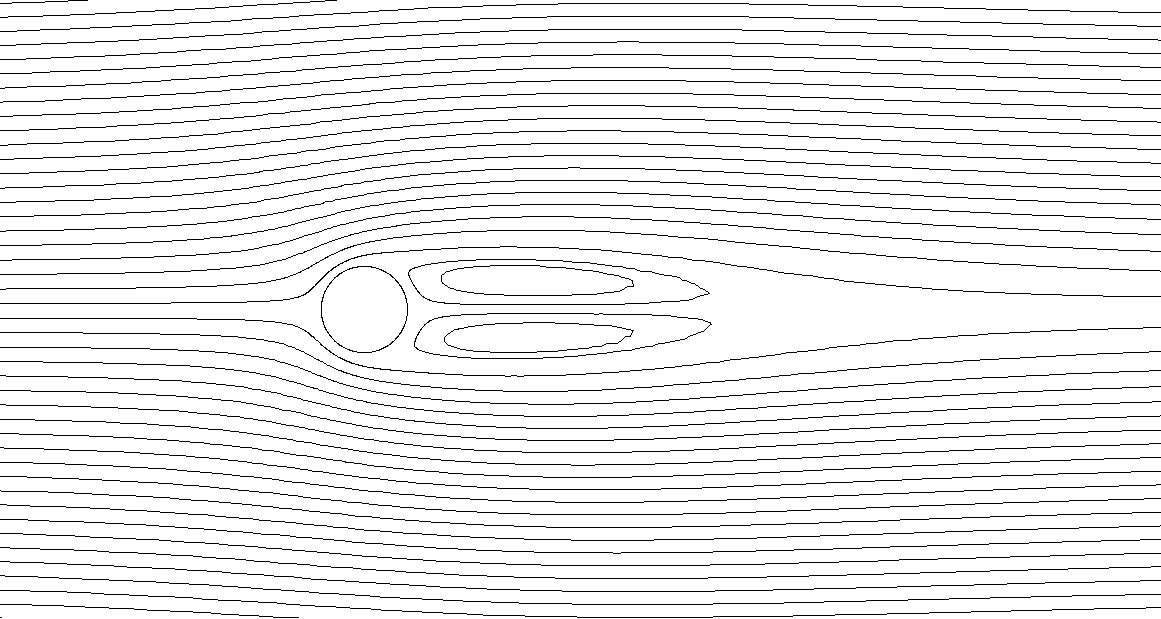
\includegraphics[height=0.2\textwidth]{Stroomfunctie_Re100_bw.png} 
	} \quad
	\subfigure[Re = 1000]{
		\label{fig:cilinder Re 1000}
		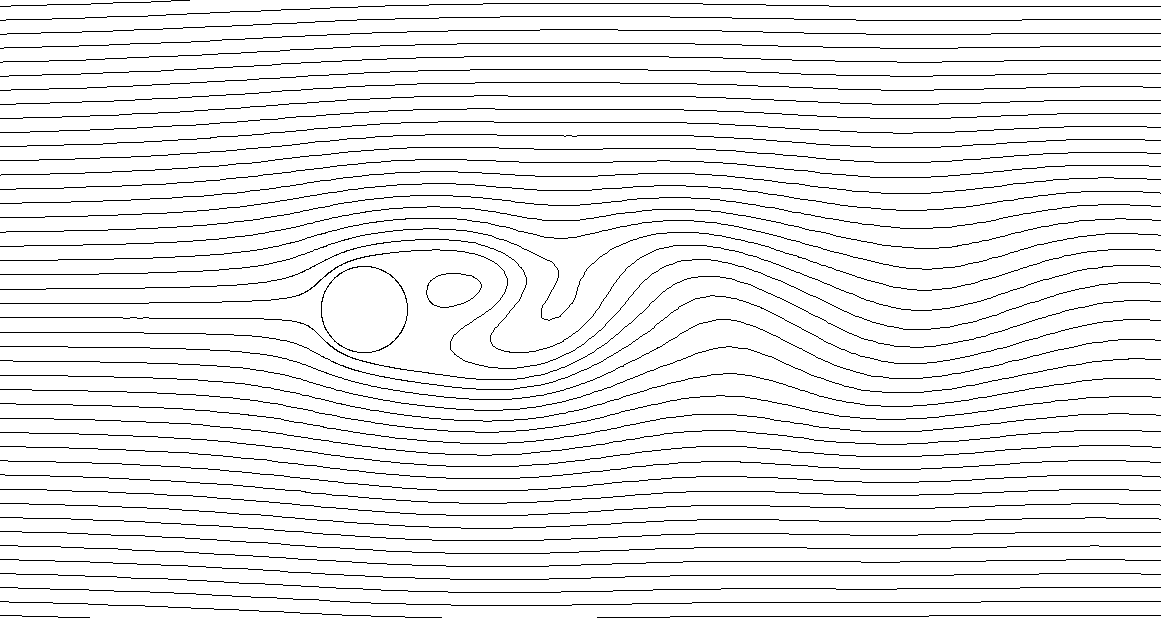
\includegraphics[height=0.2\textwidth]{Stroomfunctie_Re1000_bw.png}
	}
	\\
	\subfigure[Re = 100000]{
		\label{fig:cilinder Re 100000}
		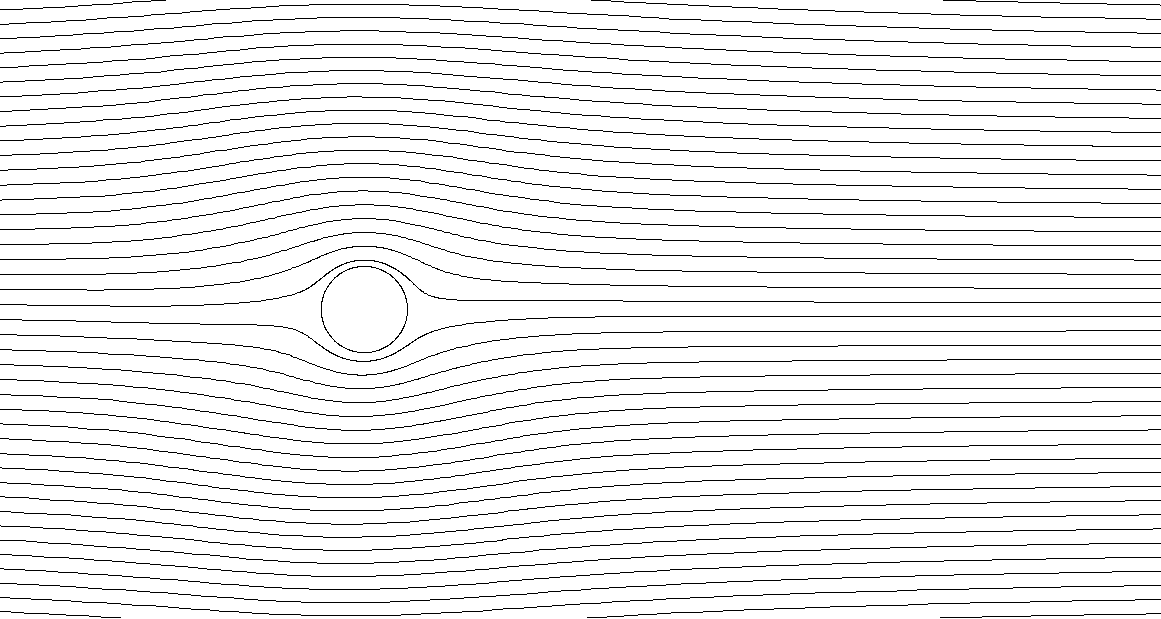
\includegraphics[height=0.2\textwidth]{Stroomfunctie_Re10000_bw.png}
	}
	\caption{Stroomlijnen bij stroming rond een cilinder voor verschillende Reynolds getallen}
	\label{fig:Sroomlijnen bij stroming rond een cilinder}
\end{figure}

Bij hogere Reynoldsgetallen zien we dat er een zog met circulatie stroming achter de cilinder ontstaat (Figuur \ref{fig:cilinder Re 100}). De wrijvingscoëfficiënt daalt ook niet meer zo sterk als verwacht onder invloed van de dalende viskeuze krachten. Dit verschijnsel wordt \emph{afscheiding} of \emph{loshechting} genoemd. Bij gemiddeld grote Reynolds getallen zal het gedeelte waarin afscheiding optreedt stabiel zijn. Bij hogere Reynolds getallen zal de stroming beurtelings langs de ene en de andere zijde loshechten waardoor er wervelingen ontstaan die zich in de stroming voortplanten (Figuur \ref{fig:cilinder Re 1000}). Deze periodische loshechting brengt een periodische kracht loodrecht op de gemiddelde stroomrichting met zich mee. De frequentie van het loshechten kan gekarakteriseerd worden door het Strouhal getal ($\text{St} = fD/v$) dat voor de stroming rond een cilinder ongeveer 0.2 is.

Bij nog hogere waarden van het Reynolds getal zal de afgescheiden zone achter de cilinder terug verkleinen terwijl ook de wrijvingscoëfficiënt terug daalt (Figuur \ref{fig:cilinder Re 100000}).

Om deze waarnemingen te verklaren bekijken we ook de stroming bij de afwezigheid van viskeuze krachten (potentiaalstroming). In deze situatie ontstaat er een hoge druk zone voor de cilinder met een stagnatiepunt waar de stroming helemaal tot stilstand komt. Aan de zijkanten (op 90\deg en 270\deg) zal de snelheid van het fluïdum het grootst zijn. De druk is hier minimaal. wanneer we verderop in de stroming kijken zal aan de achterzijde van de cilinder (180\deg) ook een stagnatiepunt zijn waar de snelheid $0$ is en de druk maximaal. Er wordt met andere woorden energie omgezet van druk aan de voorzijde van de cilinder naar kinetische energie aan de randen en terug naar druk aan de achterzijde van de cilinder. Aan de achterzijde van de cilinder zal de druk stijgen, er heerst een positieve drukgradiënt.

Hetzelfde geldt voor het niet viskeuze gedeelte (het gedeelte buiten de grenslaag) van de bovenstaande stromingen. Uit de grenslaag theorie volgt dat er binnen de grenslaag geen drukvariaties met de hoogte zijn. Aan de achterzijde van de cilinder vinden we dus ook binnen de grenslaag een positieve drukgradiënt. Binnen de grenslaag wordt er echter ook energie gedissipieerd door de viskeuze wrijving. De stroming zal dus voor het normale stagnatiepunt ($\theta = 180\deg$) tot stilstand komen. Aangezien er buiten de grenslaag wel nog steeds een positieve drukgradiënt heerst zal de stroming binnen de grenslaag zelfs van richting veranderen en terugstromen over het oppervlak van de cilinder (\ref{fig:afscheiding}).

Bij hogere Reynoldsgetallen zal het gebied in afscheiding terug afnemen. Dit wordt veroorzaakt doordat de stroming turbulent wordt aan het oppervlak van de cilinder. Bij turbulente stroming is de convectieve impulsoverdracht veel groter (het snelheidsprofiel wordt vlakker) er wordt dus meer energie van de vrije stroming naar de grenslaag overgedragen zodat de drukstijging gemakkelijker overwonnen kan worden. Aan de achterzijde van de cilinder ontstaat een turbulent zog. Bij nog hogere Reynoldsgetallen zal dit zog terug uitbreiden wanneer de volledige grenslaag turbulent wordt.

%%%%%%%%%%%%%%%%%%%%%%%%%%%%%%%%%%%%%%%%%%%%%%%%%%%%%%%%%%%%%%%%%%%%%%%%%%%%%%%%%%%%%
	\section{Stroming rond een vleugelprofiel}
	\label{sec:Stroming rond een vleugelprofiel}

Een in de ingenieurstoepassingen veel voorkomend voorwerp is een vleugelprofiel. Onder de term vleugelprofiel vallen alle voorwerpen waarvan het doel is dat wanneer ze door een stroming bewegen ze een kracht loodrecht op de stroming ondervinden. Een vleugelprofiel zal dus niet enkel een \emph{weerstandskracht} in de richting van de stroming ondervinden maar ook een kracht loodrecht op de stroming, de \emph{liftkracht} (Figuur \ref{fig:vleugelprofiel krachten}).
\begin{figure}[htb]
	\centering
	\includegraphics{fig/uitwendige_stroming/vleugelprofiel_krachten}
	\caption{Weerstandskracht en liftkracht op een vleugelprofiel}
	\label{fig:vleugelprofiel krachten}
\end{figure}

Wanneer we de stoomlijnen van een stationaire stroming rond een vleugelprofiel visualiseren (Figuur \ref{fig:vleugelprofiel stroomlijnen}) Zien we dat de stroming door het profiel naar beneden afgebogen wordt. Volgens de wet van behoud van impuls (\ref{eqn:controlevolume,behoud van impuls}) zal de stroming dus een verticale reactiekracht op het profiel uitoefenen.
\begin{figure}[htb]
	\centering
	\includegraphics{fig/uitwendige_stroming/vleugelprofiel_stroomlijnen}
	\caption{Stroomlijnen rond een vleugelprofiel}
	\label{fig:vleugelprofiel stroomlijnen}
\end{figure}
De liftkracht en een gedeelte van de weerstandskracht worden door de druk in de stroming uitgeoefend op het profiel. Wanneer we deze druk uitzetten op over profiel (Figuur \ref{fig:vleugelprofiel drukverdeling}) zien we dat aan de bovenzijde er een onderdruk heerst terwijl er aan de onderzijde overdruk heerst. Aan de wand van het vleugelprofiel zal ook een grenslaag ontstaan die naargelang het Reynoldsgetal van de stroming laminair of turbulent kan zijn.
\begin{figure}[htb]
	\centering
	\includegraphics{fig/uitwendige_stroming/vleugelprofiel_drukverdeling}
	\caption{Drukverdeling rond een vleugelprofiel}
	\label{fig:vleugelprofiel drukverdeling}
\end{figure}

De grootte van de lift- en weerstandskracht die gegenereerd worden door het profiel zullen afhangen van de mate waarin de stroming afgebogen wordt. De afbuiging zal sterk afhangen van hoek die het profiel maakt met de vrije stroomrichting.
De \emph{koorde} van een profiel wordt gedefinieerd als de verbindingslijn tussen de aanvalsboord en de achterrand. We kunnen nu de aanvalshoek definiëren als de hoek $\alpha$ tussen de koorde en de vrije stroomsnelheid (Figuur \ref{fig:vleugelprofiel aanvalshoek}).
\begin{figure}[htb]
	\centering
	\includegraphics{fig/uitwendige_stroming/vleugelprofiel_aanvalshoek}
	\caption{Koorde en aanvalshoek bij een vleugelprofiel}
	\label{fig:vleugelprofiel aanvalshoek}
\end{figure}
We kunnen nu de lift en weerstandskracht uitzetten ten opzichte van de aanvalshoek. We kunnen deze krachten onafhankelijk van de snelheid weergeven als twee krachtcoëfficiënten, de liftcoëfficiënt en de weerstands- of dragcoëfficiënt
\begin{eqnarray}
	C_d &=& \dfrac{F_d}{\frac{1}{2}\rho v_{\infty}^2 A} \\
	C_l &=& \dfrac{F_l}{\frac{1}{2}\rho v_{\infty}^2 A}
\end{eqnarray}
Aangezien deze krachten sterk afhankelijk van de aanvalshoek zullen zijn moeten we de krachtcoëfficiënten onafhankelijk van de aanvalshoek definiëren. Dit kunnen we door het oppervlak $A$ onafhankelijk van de aanvalshoek te kiezen als de koorde $c$ maal de lengte $L$ van het profiel:
\begin{eqnarray}
	A = c L
\end{eqnarray}
Wanneer we de lift- een weerstandscoëfficiënten uitzetten ten opzichte van de aanvalshoek krijgen we het resultaat van Figuur \ref{fig:lift en weerstand ifv aanvalshoek}.
\begin{figure}[htb]
	\centering
	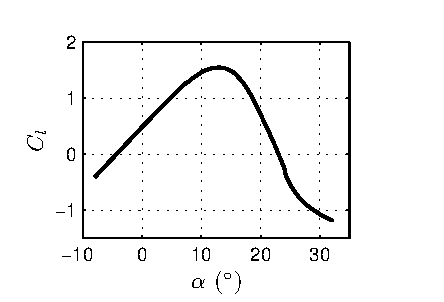
\includegraphics{NACA_4412_Cl.pdf}
	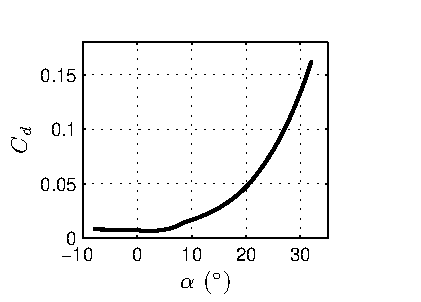
\includegraphics{NACA_4412_Cd.pdf}
	\caption{lift- een weerstandscoëfficiënten van een NACA 4412 profiel bij variërende aanvalshoek}
	\label{fig:lift en weerstand ifv aanvalshoek}
\end{figure}

Bij kleine aanvalshoeken zien we dat de liftcoëfficiënt ongeveer lineair stijgt met de aanvalshoek. tewijl de weerstandscoëfficiënt langzaam stijgt. Vanaf een gegeven aanvalshoek zal de liftkracht niet meer stijgen en op een gegeven moment terug beginnen dalen. Tegelijk stijgt de weerstandscoëfficiënt sterk. Dit gebeurt bij een hoek die veel kleiner is dan we zouden verwachten door middel van behoud van impuls.

Aan de bovenzijde van het profiel heerst een onderdruk die net na de aanvalsboord het grootst is. Aan de achterzijde van het profiel is de druk ongeveer de omgevingsdruk. Er is dus een stijgende druk aan de bovenzijde van het profiel. In combinatie met de gevormde grenslaag zorgt dit ervoor dat de stroming zal loshechten van het profiel. Er ontstaat een zog op omgevingsdruk dat ervoor zorgt dat de lift vermindert en de weerstand stijgt.

De weerstandkracht die aangrijpt op het profiel kan opgesplitst worden in 2 componenten. De aanwezigheid van een grenslaag impliceert dat er schuifspanningen op het oppervlak zullen uitgeoefend worden. Deze resulteren in viskeuse weerstand (E: Viscous drag, skin friction). Deze vorm van weerstand is dominant bij voorwerpen die een aanzienlijke oppervlakte hebben maar waar deze oppervlakte voornamelijk in de richting van de stroming georiënteerd is of gestroomlijnde voorwerpen.

Wanneer we de drukverdeling rond het vleugelprofiel in Figuur \ref{fig:vleugelprofiel drukverdeling} bestuderen valt op dat de druk aan de aanvalsboord van het profiel groter is dan aan de achterzijde. Deze variatie zal ook resulteren in een kracht in de richting van de stroming, een weerstandskracht dus. We noemen dit vormweerstand (E: form drag, pressure drag). Bij voorwerpen die niet gestroomlijnd zijn of stompe voorwerpen zal deze vorm van weerstandskracht domineren.

We zien dus dat bij vleugelprofielen beide vormen van weerstandskracht terugkomen. Bij kleine aanvalshoeken is het vleugelprofiel een zeer gestroomlijnd voorwerp en zal de vormweerstand zeer klein zijn. De viskeuse weerstand blijft echter aanwezig. Bij grotere aanvalshoeken zal het vleugelprofiel zich meer en meer gedragen als een stomp voorwerp en wordt de vormweerstand veel belangrijker dan de viskeuse weerstand. In het diagram voor de weerstandscoëfficiënt van Figuur \ref{fig:lift en weerstand ifv aanvalshoek} is dit duidelijk terug te vinden. Bij kleine aanvalshoeken blijft de weerstandscoëfficiënt quasi constant, bij grotere hoeken stijgt deze zeer snel.

Ook bij andere voorwerpen dan vleugelprofielen is de weerstandskracht steeds op te splitsen in een viskeus deel en een vorm component.

Uit de gelijkvormigheidstheorie weten we verder dat de krachten ook afhankelijk zullen zijn van het Reynolds getal: 
\begin{eqnarray}
	C_d &=& C_d(\text{Re}) \\
	C_l &=& C_l(\text{Re})
\end{eqnarray}
Deze effecten komen echter pas tot uiting bij verandering van het Reynoldsgetal over meerdere grootte ordes en hoeven bij de meeste toepassingen niet in rekening worden gebracht.
